% Generated by Sphinx.
\def\sphinxdocclass{report}
\documentclass[letterpaper,10pt,english]{sphinxmanual}
\usepackage[utf8]{inputenc}
\DeclareUnicodeCharacter{00A0}{\nobreakspace}
\usepackage[T1]{fontenc}
\usepackage{babel}
\usepackage{times}
\usepackage[Bjarne]{fncychap}
\usepackage{longtable}
\usepackage{sphinx}
\usepackage{multirow}
\DeclareUnicodeCharacter{672C}{X}


\title{Bibulous Documentation}
\date{November 14, 2013}
\release{1.2}
\author{Bibulous developers}
\newcommand{\sphinxlogo}{
\includegraphics{banner.pdf}\par}
\renewcommand{\releasename}{Release}
\makeindex

\makeatletter
\def\PYG@reset{\let\PYG@it=\relax \let\PYG@bf=\relax%
    \let\PYG@ul=\relax \let\PYG@tc=\relax%
    \let\PYG@bc=\relax \let\PYG@ff=\relax}
\def\PYG@tok#1{\csname PYG@tok@#1\endcsname}
\def\PYG@toks#1+{\ifx\relax#1\empty\else%
    \PYG@tok{#1}\expandafter\PYG@toks\fi}
\def\PYG@do#1{\PYG@bc{\PYG@tc{\PYG@ul{%
    \PYG@it{\PYG@bf{\PYG@ff{#1}}}}}}}
\def\PYG#1#2{\PYG@reset\PYG@toks#1+\relax+\PYG@do{#2}}

\expandafter\def\csname PYG@tok@gd\endcsname{\def\PYG@tc##1{\textcolor[rgb]{0.63,0.00,0.00}{##1}}}
\expandafter\def\csname PYG@tok@gu\endcsname{\let\PYG@bf=\textbf\def\PYG@tc##1{\textcolor[rgb]{0.50,0.00,0.50}{##1}}}
\expandafter\def\csname PYG@tok@gt\endcsname{\def\PYG@tc##1{\textcolor[rgb]{0.00,0.25,0.82}{##1}}}
\expandafter\def\csname PYG@tok@gs\endcsname{\let\PYG@bf=\textbf}
\expandafter\def\csname PYG@tok@gr\endcsname{\def\PYG@tc##1{\textcolor[rgb]{1.00,0.00,0.00}{##1}}}
\expandafter\def\csname PYG@tok@cm\endcsname{\let\PYG@it=\textit\def\PYG@tc##1{\textcolor[rgb]{0.25,0.50,0.56}{##1}}}
\expandafter\def\csname PYG@tok@vg\endcsname{\def\PYG@tc##1{\textcolor[rgb]{0.73,0.38,0.84}{##1}}}
\expandafter\def\csname PYG@tok@m\endcsname{\def\PYG@tc##1{\textcolor[rgb]{0.13,0.50,0.31}{##1}}}
\expandafter\def\csname PYG@tok@mh\endcsname{\def\PYG@tc##1{\textcolor[rgb]{0.13,0.50,0.31}{##1}}}
\expandafter\def\csname PYG@tok@cs\endcsname{\def\PYG@tc##1{\textcolor[rgb]{0.25,0.50,0.56}{##1}}\def\PYG@bc##1{\setlength{\fboxsep}{0pt}\colorbox[rgb]{1.00,0.94,0.94}{\strut ##1}}}
\expandafter\def\csname PYG@tok@ge\endcsname{\let\PYG@it=\textit}
\expandafter\def\csname PYG@tok@vc\endcsname{\def\PYG@tc##1{\textcolor[rgb]{0.73,0.38,0.84}{##1}}}
\expandafter\def\csname PYG@tok@il\endcsname{\def\PYG@tc##1{\textcolor[rgb]{0.13,0.50,0.31}{##1}}}
\expandafter\def\csname PYG@tok@go\endcsname{\def\PYG@tc##1{\textcolor[rgb]{0.19,0.19,0.19}{##1}}}
\expandafter\def\csname PYG@tok@cp\endcsname{\def\PYG@tc##1{\textcolor[rgb]{0.00,0.44,0.13}{##1}}}
\expandafter\def\csname PYG@tok@gi\endcsname{\def\PYG@tc##1{\textcolor[rgb]{0.00,0.63,0.00}{##1}}}
\expandafter\def\csname PYG@tok@gh\endcsname{\let\PYG@bf=\textbf\def\PYG@tc##1{\textcolor[rgb]{0.00,0.00,0.50}{##1}}}
\expandafter\def\csname PYG@tok@ni\endcsname{\let\PYG@bf=\textbf\def\PYG@tc##1{\textcolor[rgb]{0.84,0.33,0.22}{##1}}}
\expandafter\def\csname PYG@tok@nl\endcsname{\let\PYG@bf=\textbf\def\PYG@tc##1{\textcolor[rgb]{0.00,0.13,0.44}{##1}}}
\expandafter\def\csname PYG@tok@nn\endcsname{\let\PYG@bf=\textbf\def\PYG@tc##1{\textcolor[rgb]{0.05,0.52,0.71}{##1}}}
\expandafter\def\csname PYG@tok@no\endcsname{\def\PYG@tc##1{\textcolor[rgb]{0.38,0.68,0.84}{##1}}}
\expandafter\def\csname PYG@tok@na\endcsname{\def\PYG@tc##1{\textcolor[rgb]{0.25,0.44,0.63}{##1}}}
\expandafter\def\csname PYG@tok@nb\endcsname{\def\PYG@tc##1{\textcolor[rgb]{0.00,0.44,0.13}{##1}}}
\expandafter\def\csname PYG@tok@nc\endcsname{\let\PYG@bf=\textbf\def\PYG@tc##1{\textcolor[rgb]{0.05,0.52,0.71}{##1}}}
\expandafter\def\csname PYG@tok@nd\endcsname{\let\PYG@bf=\textbf\def\PYG@tc##1{\textcolor[rgb]{0.33,0.33,0.33}{##1}}}
\expandafter\def\csname PYG@tok@ne\endcsname{\def\PYG@tc##1{\textcolor[rgb]{0.00,0.44,0.13}{##1}}}
\expandafter\def\csname PYG@tok@nf\endcsname{\def\PYG@tc##1{\textcolor[rgb]{0.02,0.16,0.49}{##1}}}
\expandafter\def\csname PYG@tok@si\endcsname{\let\PYG@it=\textit\def\PYG@tc##1{\textcolor[rgb]{0.44,0.63,0.82}{##1}}}
\expandafter\def\csname PYG@tok@s2\endcsname{\def\PYG@tc##1{\textcolor[rgb]{0.25,0.44,0.63}{##1}}}
\expandafter\def\csname PYG@tok@vi\endcsname{\def\PYG@tc##1{\textcolor[rgb]{0.73,0.38,0.84}{##1}}}
\expandafter\def\csname PYG@tok@nt\endcsname{\let\PYG@bf=\textbf\def\PYG@tc##1{\textcolor[rgb]{0.02,0.16,0.45}{##1}}}
\expandafter\def\csname PYG@tok@nv\endcsname{\def\PYG@tc##1{\textcolor[rgb]{0.73,0.38,0.84}{##1}}}
\expandafter\def\csname PYG@tok@s1\endcsname{\def\PYG@tc##1{\textcolor[rgb]{0.25,0.44,0.63}{##1}}}
\expandafter\def\csname PYG@tok@gp\endcsname{\let\PYG@bf=\textbf\def\PYG@tc##1{\textcolor[rgb]{0.78,0.36,0.04}{##1}}}
\expandafter\def\csname PYG@tok@sh\endcsname{\def\PYG@tc##1{\textcolor[rgb]{0.25,0.44,0.63}{##1}}}
\expandafter\def\csname PYG@tok@ow\endcsname{\let\PYG@bf=\textbf\def\PYG@tc##1{\textcolor[rgb]{0.00,0.44,0.13}{##1}}}
\expandafter\def\csname PYG@tok@sx\endcsname{\def\PYG@tc##1{\textcolor[rgb]{0.78,0.36,0.04}{##1}}}
\expandafter\def\csname PYG@tok@bp\endcsname{\def\PYG@tc##1{\textcolor[rgb]{0.00,0.44,0.13}{##1}}}
\expandafter\def\csname PYG@tok@c1\endcsname{\let\PYG@it=\textit\def\PYG@tc##1{\textcolor[rgb]{0.25,0.50,0.56}{##1}}}
\expandafter\def\csname PYG@tok@kc\endcsname{\let\PYG@bf=\textbf\def\PYG@tc##1{\textcolor[rgb]{0.00,0.44,0.13}{##1}}}
\expandafter\def\csname PYG@tok@c\endcsname{\let\PYG@it=\textit\def\PYG@tc##1{\textcolor[rgb]{0.25,0.50,0.56}{##1}}}
\expandafter\def\csname PYG@tok@mf\endcsname{\def\PYG@tc##1{\textcolor[rgb]{0.13,0.50,0.31}{##1}}}
\expandafter\def\csname PYG@tok@err\endcsname{\def\PYG@bc##1{\setlength{\fboxsep}{0pt}\fcolorbox[rgb]{1.00,0.00,0.00}{1,1,1}{\strut ##1}}}
\expandafter\def\csname PYG@tok@kd\endcsname{\let\PYG@bf=\textbf\def\PYG@tc##1{\textcolor[rgb]{0.00,0.44,0.13}{##1}}}
\expandafter\def\csname PYG@tok@ss\endcsname{\def\PYG@tc##1{\textcolor[rgb]{0.32,0.47,0.09}{##1}}}
\expandafter\def\csname PYG@tok@sr\endcsname{\def\PYG@tc##1{\textcolor[rgb]{0.14,0.33,0.53}{##1}}}
\expandafter\def\csname PYG@tok@mo\endcsname{\def\PYG@tc##1{\textcolor[rgb]{0.13,0.50,0.31}{##1}}}
\expandafter\def\csname PYG@tok@mi\endcsname{\def\PYG@tc##1{\textcolor[rgb]{0.13,0.50,0.31}{##1}}}
\expandafter\def\csname PYG@tok@kn\endcsname{\let\PYG@bf=\textbf\def\PYG@tc##1{\textcolor[rgb]{0.00,0.44,0.13}{##1}}}
\expandafter\def\csname PYG@tok@o\endcsname{\def\PYG@tc##1{\textcolor[rgb]{0.40,0.40,0.40}{##1}}}
\expandafter\def\csname PYG@tok@kr\endcsname{\let\PYG@bf=\textbf\def\PYG@tc##1{\textcolor[rgb]{0.00,0.44,0.13}{##1}}}
\expandafter\def\csname PYG@tok@s\endcsname{\def\PYG@tc##1{\textcolor[rgb]{0.25,0.44,0.63}{##1}}}
\expandafter\def\csname PYG@tok@kp\endcsname{\def\PYG@tc##1{\textcolor[rgb]{0.00,0.44,0.13}{##1}}}
\expandafter\def\csname PYG@tok@w\endcsname{\def\PYG@tc##1{\textcolor[rgb]{0.73,0.73,0.73}{##1}}}
\expandafter\def\csname PYG@tok@kt\endcsname{\def\PYG@tc##1{\textcolor[rgb]{0.56,0.13,0.00}{##1}}}
\expandafter\def\csname PYG@tok@sc\endcsname{\def\PYG@tc##1{\textcolor[rgb]{0.25,0.44,0.63}{##1}}}
\expandafter\def\csname PYG@tok@sb\endcsname{\def\PYG@tc##1{\textcolor[rgb]{0.25,0.44,0.63}{##1}}}
\expandafter\def\csname PYG@tok@k\endcsname{\let\PYG@bf=\textbf\def\PYG@tc##1{\textcolor[rgb]{0.00,0.44,0.13}{##1}}}
\expandafter\def\csname PYG@tok@se\endcsname{\let\PYG@bf=\textbf\def\PYG@tc##1{\textcolor[rgb]{0.25,0.44,0.63}{##1}}}
\expandafter\def\csname PYG@tok@sd\endcsname{\let\PYG@it=\textit\def\PYG@tc##1{\textcolor[rgb]{0.25,0.44,0.63}{##1}}}

\def\PYGZbs{\char`\\}
\def\PYGZus{\char`\_}
\def\PYGZob{\char`\{}
\def\PYGZcb{\char`\}}
\def\PYGZca{\char`\^}
\def\PYGZam{\char`\&}
\def\PYGZlt{\char`\<}
\def\PYGZgt{\char`\>}
\def\PYGZsh{\char`\#}
\def\PYGZpc{\char`\%}
\def\PYGZdl{\char`\$}
\def\PYGZti{\char`\~}
% for compatibility with earlier versions
\def\PYGZat{@}
\def\PYGZlb{[}
\def\PYGZrb{]}
\makeatother

\begin{document}

\maketitle
\tableofcontents
\phantomsection\label{index::doc}


Contents:


\chapter{Getting started}
\label{getting_started:bibulous-documentation}\label{getting_started:getting-started}\label{getting_started::doc}
For general users, all that is needed is place the main \code{bibulous.py} file into the Python path and to tell LaTeX to use Bibulous rather than BibTeX as their bibliography engine. For users interested in using the auxiliary command \code{bibulous\_authorextract.py}, this file must also be in the Python path, and must be in the same directory as the main file.


\section{Kile: replacing BibTeX with Bibulous}
\label{getting_started:kile-replacing-bibtex-with-bibulous}\begin{enumerate}
\item {} 
In your \code{.tex} file, change the filename of the \code{\textbackslash{}bibliography\{...\}} command to the filename for the appropriate Bibulous-format bibliography style template (\code{.bst} file).

\item {} 
In Kile, go to the menu bar and select \code{Settings} \textgreater{} \code{Configure Kile}. Select \code{Tools} \textgreater{} \code{Build} and choose \code{BibTeX} from the \code{Select a tool} menu (see the figure). To the right of the menu, after you select \code{BibTeX} you should see ``Choose a configuration for the tool BibTeX''. Below the drop-down menu, select the button ``New'' and type in the name \code{Bibulous} (or whatever you prefer to call your new tool). Below, in the \code{General} tab, type in the location of the \code{bibulous.py} file. And in the \code{Options} field, type \code{\%dir\_base/\%S.aux}.

\end{enumerate}

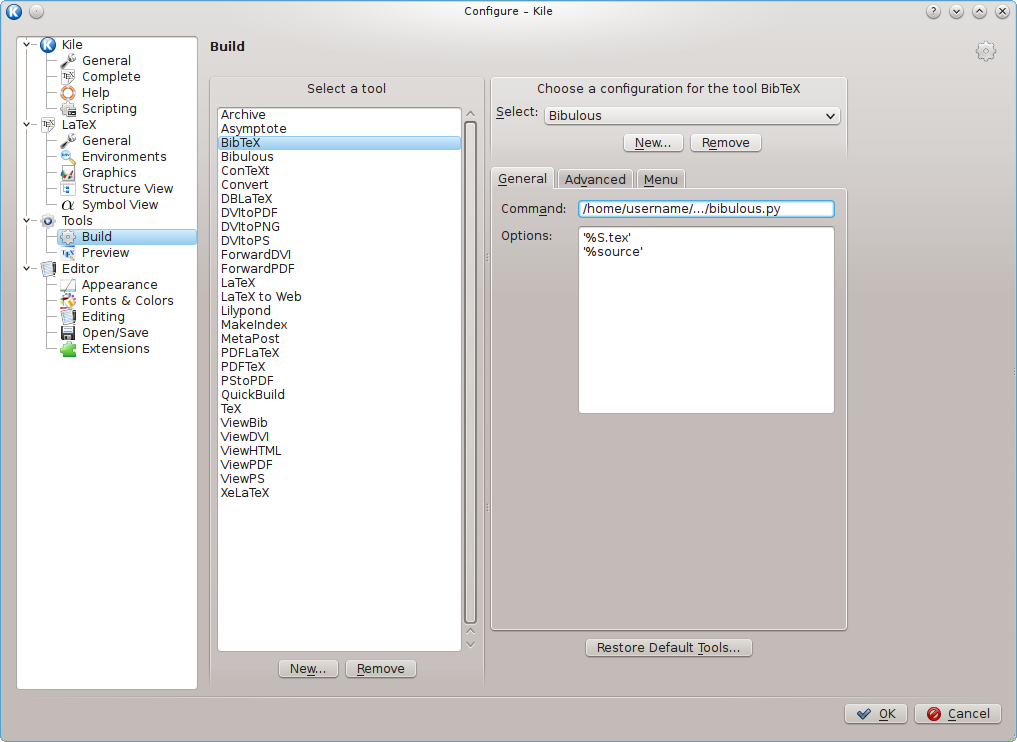
\includegraphics[width=0.490\linewidth]{screenshot_for_kile_instructions.png}

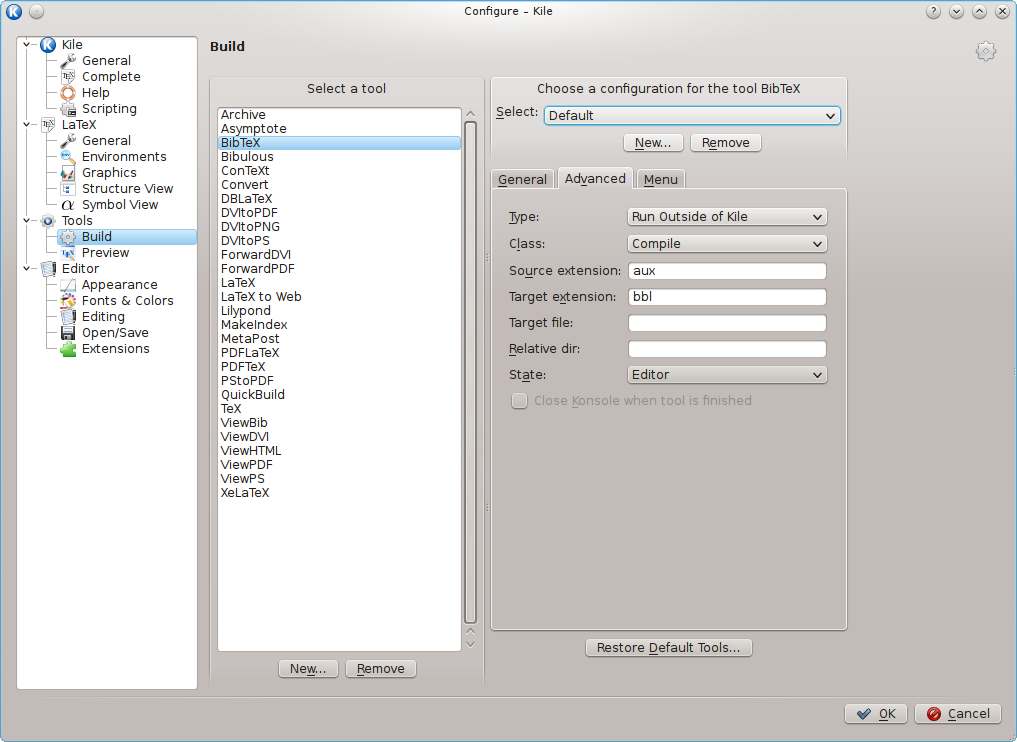
\includegraphics[width=0.490\linewidth]{screenshot_for_kile_instructions2.png}

That should be it. In case your default setup is different, you can also check the \code{Advanced} tab settings and verify that they are as shown in the second figure. (That is, \code{Source extension} is set to \code{aux}, and \code{Target extension} is set to \code{bbl}.)
\begin{enumerate}
\setcounter{enumi}{2}
\item {} 
Note that the following variables are accessible in Kile's \code{Options} field:

\begin{Verbatim}[commandchars=\\\{\}]
\%source = filename (i.e. filename with suffix but not path)
\%S = filename without suffix (and without path)
\%dir\_base = source file directory (source file's path without the filename)
\%dir\_target = target file directory (source file's path without the filename)
\end{Verbatim}

\end{enumerate}


\section{Modifying WinEdt5 to replace BibTeX with Bibulous}
\label{getting_started:modifying-winedt5-to-replace-bibtex-with-bibulous}\begin{enumerate}
\item {} 
Go to the menu \code{Options} \textgreater{} \code{Execution Modes}. In the \code{Console Applications} menu on the left hand side, select \code{BibTeX}. Then replace the three \code{Command Line} fields with the ones shown in the figure, replacing the files paths with the ones correct for your installation of Python and \code{bibulous.py}.

\end{enumerate}

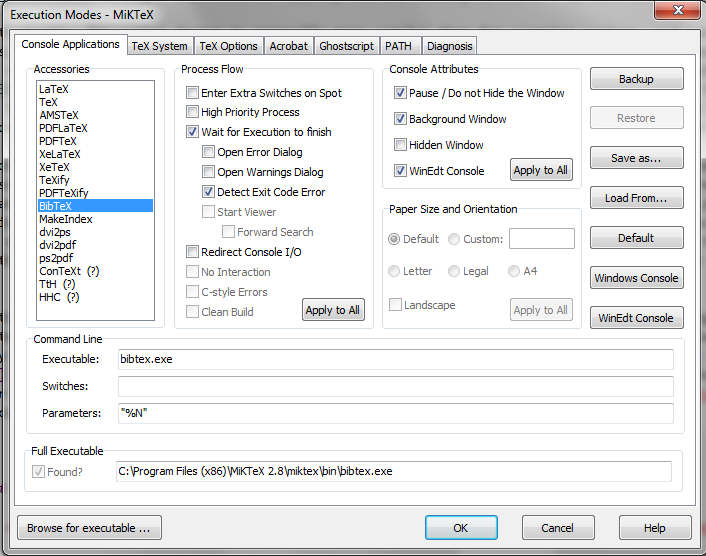
\includegraphics[width=0.490\linewidth]{original_Winedt5_setup.png}

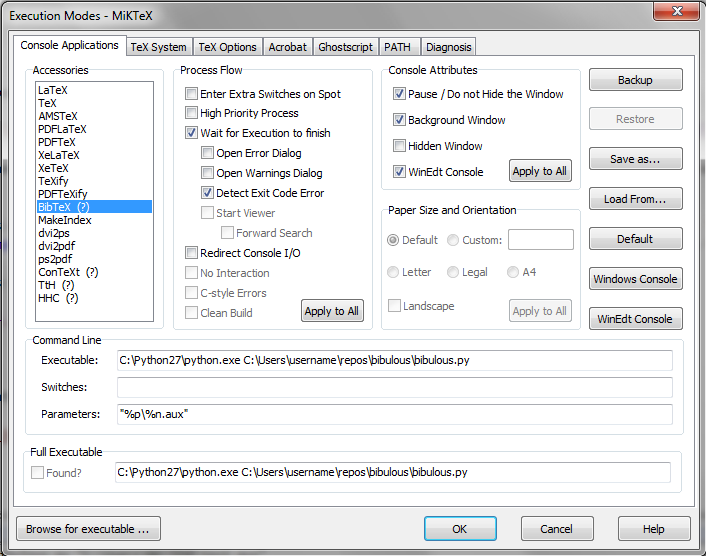
\includegraphics[width=0.490\linewidth]{modified_Winedt5_setup.png}
\begin{enumerate}
\setcounter{enumi}{1}
\item {} 
Note that the following are definitions of WinEdt registers:

\begin{Verbatim}[commandchars=\\\{\}]
\%f = full path of active file (= \%p/\%n.\%t)
\%n = name of the active file
\%p = the path of the active file
\%t = the extension of the active file
\%q = the path relative to the main file (i.e. for subdirectories)
\%b = WinEdt's local working directory (not the tex file directory)
\%B = path to the WinEdt executable file
\end{Verbatim}

\end{enumerate}


\chapter{Guidelines for writing bibliography style templates}
\label{guidelines_for_writing_style_templates:guidelines-for-writing-bibliography-style-templates}\label{guidelines_for_writing_style_templates::doc}\begin{enumerate}
\item {} 
Comments begin with \code{\#}. (A single \code{\#} indicates a symbol and not a comment!)

\item {} 
A line which begins with an entrytype name followed by an \code{=} sign defines the bibliographic format for that entrytype. For example:

\begin{Verbatim}[commandchars=\\\{\}]
article = \textless{}authorlist\textgreater{}, {}`{}`\textless{}title\textgreater{},'' \textless{}journal\textgreater{}, \textless{}volume\textgreater{}, ...
           [\textless{}startpage\textgreater{}--\textless{}endpage\textgreater{}\textbar{}\textless{}eid\textgreater{}\textbar{}]  (\textless{}year\textgreater{}). [\textless{}note\textgreater{}.]
\end{Verbatim}

Here the \code{article} entrytype will be typeset so that the list of authors is followed by the article title in double quotes, the journal name in standard font (i.e. not italics), the volume number, the page range, and the year.

\item {} 
Square brackets \code{{[}{]}} indicate an optional entry; any required entries which are not defined in the BibTeX database file (.bib file) are replaced with `???' by default. Optional arguments is undefined are simply skipped. If a \code{\textbar{}} is present within the square brackets, it indicates an ``elseif'' argument (if not the final \code{\textbar{}} within the brackets), or an ``else'' argument (if the final \code{\textbar{}}). The ``else'' indicates a \emph{required} argument, so if you want an optional entry to be replaced with something, you can use \code{{[}option\textbar{}{]}} --- the use of an empty cell inside the square brackets indicates that we simply use the default replacement for an undefined required argument (i.e. \code{???}). If you want all of the cells to be optional, then use \code{\textbar{}''{]}} in the last cell -- that is, the last cell should be an empty string. For  now, the format currently does not allow nesting of brackets.

\item {} 
If you need the square brackets or \code{\textbar{}} symbol as formatting elements, then simply use \code{\{\textbackslash{}makeopenbracket\}}, \code{\{\textbackslash{}makeclosebracket\}}, or \code{\{\textbackslash{}makeverticalbar\}}. If you need the angle brackets as formatting elements, then use \code{\{\textbackslash{}makegreaterthan\}} and \code{\{\textbackslash{}makelessthan\}}. Note that the curly brackets are needed here so that when Bibulous replaces the command with the appropriate symbol, that symbol can be used correctly in LaTeX commands.

\item {} 
Unlike BibTeX, Bibulous does \emph{not} change the capitalization state of any entry variables. It assumes that the authors have defined it the way they want it.

\item {} 
If an entrytype format definition contains only another entrytype on the right hand side of the \code{=}, for example:

\begin{Verbatim}[commandchars=\\\{\}]
\PYG{n}{inbook} \PYG{o}{=} \PYG{n}{incollection}
\end{Verbatim}

then this simply defines the format for the entrytype on the left hand side as identical to that of the entrytype given on the right hand side.

\item {} 
The second type of data present in the file are the formatting options. These are defined by writing \code{options} followed by a period and then the option name, for example:

\begin{Verbatim}[commandchars=\\\{\}]
\PYG{n}{options}\PYG{o}{.}\PYG{n}{authorlist\PYGZus{}format} \PYG{o}{=} \PYG{l+s}{'}\PYG{l+s}{first\PYGZus{}name\PYGZus{}first}\PYG{l+s}{'}
\end{Verbatim}

\item {} 
Bibulous only allows string variables to be inserted into a given position within an entrytype template, and all Bibulous variables are surrounded with angle brackets. Thus, when typesetting the bibliography, Bibulous will replace the variable \code{\textless{}authorlist\textgreater{}} with the string stored in the \code{authorlist} field of the current entry being formatted. An example list of variables one may choose to use is:
\begin{quote}

\code{\textless{}authorlist\textgreater{}}, \code{\textless{}booktitle\textgreater{}}, \code{\textless{}chapter\textgreater{}}, \code{\textless{}edition\_ordinal\textgreater{}}, \code{\textless{}editorlist\textgreater{}}, \code{\textless{}eid\textgreater{}}, \code{\textless{}endpage\textgreater{}}, \code{\textless{}institution\textgreater{}}, \code{\textless{}journal\textgreater{}}, \code{\textless{}nationality\textgreater{}}, \code{\textless{}note\textgreater{}}, \code{\textless{}number\textgreater{}}, \code{\textless{}organization\textgreater{}}, \code{\textless{}publisher\textgreater{}}, \code{\textless{}school\textgreater{}}, \code{\textless{}series\textgreater{}}, \code{\textless{}startpage\textgreater{}}, \code{\textless{}title\textgreater{}}, \code{\textless{}version\textgreater{}}, \code{\textless{}volume\textgreater{}}, \code{\textless{}year\textgreater{}}.
\end{quote}

As one can see, these primarily consist of the various fields one can expect to see within a given BibTeX-formatted database file. This list is actually freely extensible. You can add whatever additional variables you like, so that if you use a special \code{video} field in your database, you can insert that field's value into the template wherever \code{\textless{}movie\textgreater{}} is located.

\item {} 
Note that several fields are defined by default which are \emph{not} directly from the bibliography database. These are \code{authorlist}, \code{editorlist}, \code{startpage}, \code{endpage}, and \code{edition\_ordinal}. These fields are derived from the original database file, but have been reformatted.

\item {} 
Although the entrytype template definitions listed below are in alphabetical order, that can be put in any desired order within the file. (The exception to this rule is that if a definition consists of, for example:

\begin{Verbatim}[commandchars=\\\{\}]
\PYG{n}{inbook} \PYG{o}{=} \PYG{n}{incollection}
\end{Verbatim}

then the \code{incollection} template must already be defined. Also note that two entrytype names are special and so cannot be used on the left hand side of the equals sign here: \code{comment} and \code{preamble}.

\item {} 
A user wanting a localized form of quotation should use \code{\textbackslash{}enquote\{\textless{}title\textgreater{}\}} rather than \code{{}`{}`\textless{}title\textgreater{}''}, and add \code{\textbackslash{}usepackage\{csquotes\}} to the preamble of the LaTeX document.

\end{enumerate}


\chapter{Instructions on how to report a bug to the Bibulous development team}
\label{instructions_for_reporting_bugs:instructions-on-how-to-report-a-bug-to-the-bibulous-development-team}\label{instructions_for_reporting_bugs::doc}

\section{Where to report a bug}
\label{instructions_for_reporting_bugs:where-to-report-a-bug}
Send an email to the \code{users\_mailing\_list}. Once it's confirmed as a bug, someone, possibly you, can enter it into the issue tracker. (Or if you're pretty sure about the bug, go ahead and post directly to the developers mailing list, \code{developers\_mailing\_list}. But if you're not sure, it's better to post to {[}\code{users mailing list}{]} first; someone there can tell you whether the behavior you encountered is expected or not.)


\section{How to report a bug}
\label{instructions_for_reporting_bugs:how-to-report-a-bug}
First, make sure it's a bug. If Bibulous does not behave the way you expect, look in the documentation and mailing list archives for evidence that it should behave the way you expect. If the documentation and archives do not contain enough information to tell you whether the behavior is a bug or is expected behavior, go ahead and ask on the users mailing list first \code{users\_mailing\_list}. Also check that you are running the most recent version of Bibulous. It may be that the bug has already been fixed.

Once you've established that it's a bug, the most important thing you can do is come up with a simple description and reproduction recipe. For example, if the bug, as you initially found it, involves five files over ten commits, try to make it happen with just one file and one commit. The simpler the reproduction recipe, the more likely a developer is to successfully reproduce the bug and fix it.

When you write up the reproduction recipe, don't just write a prose description of what you did to make the bug happen. Instead, give a copy of the exact series of commands you ran, and their output. Use cut-and-paste to do this. If there are files involved, be sure to include the names of the files, and even their content if you think it might be relevant. The very best thing is to package your reproduction recipe as a script, that helps a lot.

In addition to the reproduction recipe, we'll also need a complete description of the environment in which you reproduced the bug. That means:
\begin{itemize}
\item {} 
Your operating system

\item {} 
The Python version you are running under.

\item {} 
The release and/or revision of Bibulous.

\item {} 
Anything else that could possibly be relevant. Err on the side of too much information, rather than too little.

\end{itemize}

Once you have all this, you're ready to write the report. Start out with a clear description of what the bug is. That is, say how you expected Bibulous to behave, and contrast that with how it actually behaved. While the bug may seem obvious to you, it may not be so obvious to someone else, so it's best to avoid a guessing game. Follow that with the environment description, and the reproduction recipe. If you also want to include speculation as to the cause, and even suggest how the code may be modified to fix the bug, that's great.

Post all of this information to the developers mailing list, \code{developers\_mailing\_list}, or if you have already been there and been asked to file an issue, then go to the Issue Tracker and follow the instructions there.

Thanks! It's a lot of work to file an effective bug report, but a good report can save hours of a developer's time, and make the bug much more likely to get fixed.


\chapter{Developer guide}
\label{developer_guide::doc}\label{developer_guide:developer-guide}

\section{Guidelines for Python coding style}
\label{developer_guide:guidelines-for-python-coding-style}\begin{enumerate}
\item {} 
Note that one can mix 8-bit Python strings (ASCII text) with UTF-8 encoded text as long as the 8-bit string contains only ASCII characters.

\item {} 
Keep in mind when running into Unicode errors: reading a line of text from a file produces a line of bytes and not characters. To decode the bytes into a string of characters, you need to know the encoding.

\item {} 
There are a couple of minor points where the Bibulous coding standards deviates from Python's PEP8:
\begin{enumerate}
\item {} 
A line width of 120 is the standard (not 80).

\item {} 
In general, statements that evaluate to a boolean are placed within parentheses (i.e. \code{if (a \textless{} b):} rather than \code{if a \textless{} b:}).

\end{enumerate}

\item {} 
Many developers prefer to spread out code among a large number of small files, but Bibulous is currently organized in a single large file. This is partly because there is no large block of code that fits by itself so that a separate file makes sense. (Parsing of \code{.bib} files, for example, only requires a couple hundred lines.

\end{enumerate}


\section{Overall project strategy and code structure}
\label{developer_guide:overall-project-strategy-and-code-structure}
The basic function of BibTeX is to accept an \code{.aux} file as input and to produce a \code{.bbl} file as output. The \code{aux} file contains all of the citation information as well as the filenames for the bibliography database file (\code{.bib}) and the style file (\code{.bst}).

The basic program flow is as follows:
\begin{enumerate}
\item {} 
Read the \code{.aux} file and get the names of the bibliography databases (\code{.bib} files), the style templates (\code{.bst} files) to use, and the entire set of citations.

\item {} 
If an ``extracted'' database file exist, then compare the citations in the extracted database against those in the \code{.aux} file. If there are any differences, then re-extract the database. Otherwise, use the extracted database rather than the full one specified in the \code{.aux} file.

\item {} 
Read in all of the bibliography database files into one long dictionary (\emph{bibdata}), replacing any abbreviations with their full form. Cross-referenced data is \emph{not} yet inserted at this point. That is delayed until the time of writing the BBL file in order to speed up parsing.

\item {} 
Read in the Bibulous style template file as a dictionary (\emph{bstdict}).

\item {} 
Now that all the information is collected, go through each citation key, find the corresponding entry key in \emph{bibdata}. If there is crossref data, then fill in missing values here. Also create the ``special fields'' here. Finally, from the entry type, select a template from \emph{bstdict} and begin inserting the variables one-by-one into the template.

\end{enumerate}

Because the \code{.bib} file is highly structured, it is straightforward to write a parser by hand in Python: the \code{parse\_bibfile()} method converts the \code{.bib} file contents into a Python dictionary (the \code{Bibdata} class' \code{bibdata}). The \code{.aux} file is even easier to parse, and the \code{parse\_auxfile()} method converts the citation information into the \code{Bibdata} class' \code{citedict} dictionary. The \code{.bst} style template file, having its own domain specific language, is much more complicated, so that its parser is generated from a grammar written for the \code{Antlr} parser generator. (This creates Bibulous' only external dependency -- Java -- which we may be able to eliminate if we use a Python-based parser generator, such as \code{pyparsing}.)

The \code{Bibdata} class thus holds all relevant information needed to operate on a bibliography and generate the output LaTeX-formatted \code{.bbl} file.


\section{Parsing BIB files}
\label{developer_guide:parsing-bib-files}

\subsection{parse\_bibfile()}
\label{developer_guide:parse-bibfile}
The strategy for \code{parse\_bibfile()} is to find each individual bibliography entry, determine its entry type, and save all of the text between the entry's opening and closing braces as one long string, to be passed to \code{parse\_bibentry()} for parsing. To gather the entry data string, we first look for the next line that starts with \code{@}. On that line, we look for a string after the \code{@} followed by \code{\{}, where the string gives the entry type. After we know the entry type, we look for the corresponding closing brace. If we don't find it on the same line, then we read in the next line, and so forth, concatenating all of the lines into one long ``entry string'' until we encounter the corresponding closing brace. Once we have this extended ``entry string'' we feed it to \code{parse\_bibentry()} to generate the bibliography data. Once we have come to the end of a given entry, we continue reading down the file looking for the next `@' and so on.

Although this approach effectively means that we have to pass twice through the same data, dealing with brace-matching can otherwise become a mess since the BibTeX format, since it allows nested delimiters, is not directly compatible with regular expressions.


\subsection{parse\_bibentry()}
\label{developer_guide:parse-bibentry}
\code{parse\_bibentry()} only needs to worry about a single entry, and there are four possible formats for the entry string passed to the function:
\begin{enumerate}
\item {} 
If the entrytype is a comment, then skip everything, adding nothing to the database dictionary.

\item {} 
If the entrytype is a preamble, then treat the entire entry contents as a single fieldvalue. Append the string onto the \code{preamble} value in the \code{bibdata} dictionary.

\item {} 
If the entrytype is a \code{string} (i.e. an abbreviation), then there is no entrykey. Get the fieldname (abbreviation key), and the remainder of the string is a single field value (the full form of the abbreviated string. Add this key-value pair to the \code{abbrevs} dictionary.

\item {} 
If the entry is any other type, then get the entrykey, and the remainder of the string is a \emph{series} of field-value pairs.

\end{enumerate}

Once it determines which of these four options to use, \code{parse\_bibentry()} extracts the entry key (if present), separates out each of the fields (if more than one is present) and loops over each field with a call to \code{parse\_bibfield()} to extract the field key-value pairs.


\subsection{parse\_bibfield()}
\label{developer_guide:parse-bibfield}
\code{parse\_bibfield()} is the workhorse function of the BIB parsing. And because of BibTeX's method for allowing concatenation, use of abbreviation keys, and use of two different types of delimiters (\code{"..."} or \code{\{...\}}), this function is a little messy. However, for the format of a given field, there are four parsing possibilities:
\begin{enumerate}
\item {} 
If the field begins with a double quote \code{"} then scan until you find the next \code{"}. Add that to the result string. If the ending \code{"} is followed by a comma, then the field is done; return the result string. If the ending is followed by a \code{\#} then expect another field string. Scan for it and append it to the current result string.

\item {} 
If the field begins with \code{\{} then scan until you resolve the brace level. This should be followed by a comma, since no concatenation is allowed of brace-delimited fields. Otherwise issue a syntax error warning.

\item {} 
If the field begins with a \code{\#} (concatenation operator) then skip whitespace to the next character set, where you should expect a quote-delimited field. Append that to the current result string.

\item {} 
If the field begins with anything else, then the substring up until the first whitespace character represents an abbreviation key. Locate it and substitute it in. If you don't find the key in the \code{abbrevs} dictionary, give a warning and skip.

\end{enumerate}


\section{Parsing AUX files}
\label{developer_guide:parsing-aux-files}
The \code{.aux} file contains the filenames of the \code{.bib} database file and the \code{.bst} style template file, as well as the citations. The \code{get\_bibfilenames()} method scans through the \code{.aux} file and locates a line with \code{\textbackslash{}bibdata\{...\}} which contains a filename or a comma-delimited list of filenames, giving the database files. Another line with \code{\textbackslash{}bibstyle\{...\}} gives the filename or comma-delimited list of filenames for style templates. The filenames obtained are saved into the \code{filedict} attribute -- a dictionary whose keys are the file extensions \code{aux}, \code{bbl}, \code{bib}, \code{bst}, or \code{tex}.

The \code{parse\_auxfile()} method makes a second pass through the \code{.aux} file, this time looking for the citation information. (Auxiliary files are generally quite small, so taking multiple passes through them cost very little time.) Each line with \code{\textbackslash{}citation\{...\}} contains a citation key or comma-delimited list of citation keys -- each one is added into the citation dictionary (\code{citedict}), with a value corresponding to the citation order.


\section{Parsing BST files}
\label{developer_guide:parsing-bst-files}
(This part is changing at the moment, and so the documentation is not available yet.)

Note format\_bibitem() is where we compile any scripts present in the BST files. Doing it before this step basically requires that we run any script on all of the entries of the database and not just the ones that have been cited. For large databases, this can be a significant amount of extra computation. There are two different compilation steps here. The first is that, before looping over the bibitems, we compile the scripts so that any functions defined there are available to the local namespace. Second, once we're inside the loop, if the template string for the current entry has a variable which is a user-defined variable, then we have to use Python's \code{eval()} function to obtain the result of evaluating the script on the current entry.


\section{Writing the BBL file}
\label{developer_guide:writing-the-bbl-file}
Now that all the information is available to Bibulous, we can begin writing the output BBL file. First we write a few lines to the preamble, including the \code{preamble} string obtained from the \code{.bib} database files. We also create the citation list -- the citations listed in the sorting order as defined in the style template files. (This requires a surprising amount of code to get right -- see \textbf{Generating sortkeys} below.) We loop over each citation in the desired order, and insert cross-reference information to fill in missing fields, and parse each name field (see the ``Formatting names'' subsection below). The cross-referencing and name parsing steps can be delayed until later on in the processing chain, but would require more complex code to do there, so doing them here keeps the code simpler without sacrificing much speed. (The assumption here is that the citation list is small, at least in comparison to the database, so that limiting the difficult parsing to only those entries cited will allow significant improvement in speed.) Finally, at each step in the loop, we call \code{format\_bibitem()} to insert the database entry fields into the appropriate style template, incorporating any extra formatting requested by the user in the style template file.


\section{Name formatting}
\label{developer_guide:name-formatting}
One of the more complex tasks needed for parsing BIB files is to resolve the elements of name lists (typically saved in the \code{author} and \code{editor} fields). In order to know how these should be inserted into a template, it is necessary to know which parts of a given person's name correspond to the first name, the middle name(s), the ``prefix'' (or ``von part''), the last name (or ``surname''), and the ``suffix'' (such as ``Jr.'' or ``III''). These five pieces or each person's name are saved as a dictionary, so that a bibliography entry with five authors is represented in \code{\textless{}authorlist\textgreater{}} as a list of five dictionaries, and each dictionary having keys \code{first}, \code{middle}, \code{prefix}, \code{last}, and \code{suffix}.

In order to speed up parsing times, the actual mapping of the \code{author} or \code{editor} fields to \code{authorlist} or \code{editorlist} is not done until the loop over citation keys performed while writing out the BBL file. The function that product the list-of-dicts parsing result is \code{namestr\_to\_namedict(namestr)}.

The default formatting of a namelist into a string to be inserted into the template is performed by \code{format\_namelist()}.


\subsection{create\_namelist()}
\label{developer_guide:create-namelist}
A BibTeX ``name'' field can consist of three different formats of names:
\begin{enumerate}
\item {} 
A space-separated list: \code{{[}firstname middlenames suffix lastname{]}}

\item {} 
A two-element comma-separated list: \code{{[}prefix lastname, firstname middlenames{]}}

\item {} 
A three-element comma-separated list: \code{{[}prefix lastname, suffix, firstname middlenames{]}}

\end{enumerate}

So, an easy way to separate these three categories is by counting the number of commas that appear. The trickiest part here is that although we can use \code{and} as a name separator, we are only allowed to do so if \code{and} occurs at the top brace level.

In addition, in order to make name parsing more flexible for nonstandard names, Bibulous adds two more name formats to this list:
\begin{enumerate}
\setcounter{enumi}{3}
\item {} 
A four-element comma-separated list: \code{{[}firstname, middlenames, prefix, lastname{]}}

\item {} 
A five-element comma-separated list: \code{{[}firstname, middlenames, prefix, lastname, suffix{]}}

\end{enumerate}

For each name in the field, we parse the name tokens into a dictionary. We then compile all of the dictionaries into a list, ordered by the appearance of the names in the input field.


\subsection{format\_namelist()}
\label{developer_guide:format-namelist}
Given a namelist (list of dictionaries), we glue the name elements together into a single string, incorporating all of the format options selected by the user in the template file. This includes calls to \code{namedict\_to\_formatted\_namestr()}, and to \code{initialize\_name()} if converting any name tokens to initials.


\section{Generating sortkeys}
\label{developer_guide:generating-sortkeys}
If the user's style template file selects the citation order to be \code{citenum} or \code{none}, then creating the ordered citation list is as simple as listing the citation keys in order of their citation appearance, which was recorded as the value in the citation dictionary. If the user instead chooses the citation order to be \code{citekey}, then all that is needed is to sort the citation keys alphabetically. Similar operations follow for the various citation order options, but the difficult lies in correctly sorting in the presence of non-ASCII languages, and especially in the presence of LaTeX markup of non-ASCII names. For a citation sorting order that requires using author names, any LaTeX markup needs to be converted to its Unicode equivalent prior to sorting. Using unicode allows the sorting to be done with any input languages, and allows the sorting order to be locale-dependent.

\code{create\_citation\_list()} is the highest-level function for generating the citation list. For each citation key, it calls \code{generate\_sortkey()}, which is the workhorse function for including all of the various options when generating the key to use for sorting the list. A key part of the function is a call to \code{purify\_string()}, which removes unnecessary LaTeX markup elements and then calls \code{latex\_to\_utf8()} to convert LaTeX-markup non-ASCII characters to Unicode. It is only after all of these conversions that the final sorting is performed and the sorted citation list returned.


\section{Testing}
\label{developer_guide:testing}
The suite of regression tests for Bibulous consist of various template definitions and database entries designed to test individual features of the program. The basic approach of the tests is as follows:
\begin{enumerate}
\item {} 
Once a change is made to the code (to fix a bug or add functionality), the developer also adds an entry to the \code{test/test1.bib} file, where the entry's ``entrytype'' is named in such a way to give an indication of what the test is for. For example, the entry in the BIB file may be defined with:

\begin{Verbatim}[commandchars=\\\{\}]
@test\_initialize1\PYGZob{}...
\end{Verbatim}

where the developer provides an \code{author} field in the entry where one or more authors have names which are difficult to for generating initials correctly. The developer should also include at least a 1-line comment about the purpose of the entry as well. To make everything easy to find, use the entrytype as the entry's key as well. Thus, the example above would use:

\begin{Verbatim}[commandchars=\\\{\}]
@test\_initialize1\PYGZob{}test\_initialize1, ...
\end{Verbatim}

\item {} 
If the above new entry is something which can be checked with normal options settings, then the developer should add a corresponding line in the BST file defining how that new entrytype (i.e. \code{test\_initialize1}) should be formatted. If \emph{different} options settings are needed, then a new BST file is needed. Only a minimalist file is generally needed: the file can, for example, contain one line defining a new entrytype and one line to define the new option setting. You can define all of the other options if you want, but these are redundant and introduce a number of unnecessary ``overwriting option value...'' warning messages.

\item {} 
Next, the developer should add a line \code{\textbackslash{}citation\{entrytype\}} to the AUX file where the key is the key given in the new entry of the BIB file you just put in (e.g. \code{test\_initialize1}). This is the same as the entrytype to keep everything consistent.

\item {} 
Next, the developer needs to add two lines to the \code{test1\_target.bbl} file to say what the formatted result should look like. Take a look at other lines to get a feel for how these should look, and take in consideration the form of the template just added to the BST file.

\item {} 
Finally, run \code{bibulous\_test.py} to check the result. This script will load the modified BIB and BST files and will write out several formatted BBL file \code{test1.bbl} etc. It will then run a \code{diff} program on the output file versus the target BBL file to see if there are any differences between the target and actual output BBL files.

\end{enumerate}


\section{Generating the documentation}
\label{developer_guide:generating-the-documentation}
From the bibulous repository \code{doc/} subfolder, run \code{make html} to generate the HTML documentation. The result can be found in \code{doc/\_build/html/}, with \code{index.html} as the main file. To generate the PDF documentation, run \code{make latexpdf} from the \code{doc/} subfolder, with the result found at \code{doc/\_build/latex/Bibulous.pdf}.


\chapter{Bibulous Overview}
\label{index:bibulous-overview}
Bibulous is a drop-in replacement for BibTeX that makes use of style templates instead of BibTeX's BST language. The code is written in Python and, like BibTeX itself, is open source.

Bibulous developed out of frustration with the complexity of creating bibliography styles using BibTeX's obscure language, and also from the realization that because bibliographies are highly structured, one should be able to specify them simply and flexibly using a template approach. There should be no need to learn a new language just to build a bibliography style, and specifying a style should taken only a matter of minutes.

Bibulous incorporates this template approach, and at the same time implements many of the modern enhancements to BibTeX, such as the ability to work with languages other than English, better support for allowing non-standard bibliography entry types, functionality for enhanced citation styles, and increased options for author name formatting, among others. The fact that Bibulous is agnostic to the names of fields in bibliography database files (\code{.bib}) means that one can use the same database and same LaTeX commands for generating each of: a bibliography, a glossary, a publications list for a CV, an annotated bibliography, and more, all within the same file and only by specifying a different style template for each case.

Bibulous' “style template” files allow a user to visualize the entire bibliography format structure in a concise way within a single page of text. Moreover, the template is structured with its own Python-like mini-language, intended to allow uses to create flexible formatting instructions quickly and easily. The example below illustrates the simplicity of the format.


\section{Installation}
\label{index:installation}
Installing using pip::

\begin{Verbatim}[commandchars=\\\{\}]
pip install bibulous
\end{Verbatim}

Instructions for installing Bibulous, and for seamlessly integrating it into your normal LaTeX workflow, are given in the \code{INSTALL.rst} file. Users can also consult the user guide (\code{user\_guide.rst}) for further information and tutorials. A \code{FAQ} page is also available.


\section{Example}
\label{index:example}
For a very simple bibliography, consisting of only journal articles and books, a complete style template file may consist of just two lines::

\begin{Verbatim}[commandchars=\\\{\}]
article = \textless{}authorlist\textgreater{}, \PYGZbs{}enquote\PYGZob{}\textless{}title\textgreater{},\PYGZcb{} \PYGZbs{}textit\PYGZob{}\textless{}journal\textgreater{}\PYGZcb{} \PYGZbs{}textbf\PYGZob{}\textless{}volume\textgreater{}\PYGZcb{}: ...
             [\textless{}startpage\textgreater{}--\textless{}endpage\textgreater{}\textbar{}\textless{}startpage\textgreater{}\textbar{}\textless{}eid\textgreater{}\textbar{}] (\textless{}year\textgreater{}).[ \textless{}note\textgreater{}]
book = [\textless{}authorlist\textgreater{}\textbar{}\textless{}editorlist\textgreater{}\textbar{}], \PYGZbs{}textit\PYGZob{}\textless{}title\textgreater{}\PYGZcb{} (\textless{}publisher\textgreater{}, \textless{}year\textgreater{})...
             [, pp.\textasciitilde{}\textless{}startpage\textgreater{}--\textless{}endpage\textgreater{}].[ \textless{}note\textgreater{}]
\end{Verbatim}

The \code{\textless{}variable\textgreater{}} notation indicates that the corresponding bibliography entry's field is to be inserted into the template there. The \code{{[}...\textbar{}...{]}} notation behaves similar to an if...elseif statement, checking whether a given field is defined within the bibliography entry. If not defined, then it attempts to implement the instruction in the block following the next \textbar{} character.

We can read the above article template as indicating the following structure for LaTeX-formatting the cited entry in the bibliography (\code{.bib} file). For articles, we first insert the list of author names (formatted according to the default form), followed by a comma. If no \code{author} field was found in the bibliography entry, then insert \code{???} to indicate a missing required field. Next insert a quoted title, followed by an italicized journal name, and a boldface volume number (all of these are required fields). Next, if the \code{pages} field was found in the entry's database, then parse the start and end page numbers and insert them here. If the \code{pages} field indicates that there was only one page, then use that instead. Or if the \code{pages} field is not present, then check to see if the \code{eid} is defined, and use it instead. However, if none of these three possibilities are available, then insert the “missing field” indicator, \code{???}. Finally, put the year inside parentheses, and if the \code{note} field is defined in the entry, then add that to the end (following the period). If \code{note} is not defined, then just ignore it.

One can read the book template similarly, and find that it has different required and optional fields. The simplicity of the format allows one to customize databases to suit any use. For example, to use a bibliography entrytype \code{本} instead of \code{book}, then all that is necessary is to go into the template file and change \code{book} to \code{本}. Of, if you wish to add a new field, such as translator, then if it has been added to the \code{.bib} database file, one need only add some text to the template, say \code{(: \textless{}translator\textgreater{})} to insert that into every bibliography entry which has translator defined for that entrytype.


\section{Developers}
\label{index:developers}
Bibulous is a brand new project, and so it has so far been a solo effort. Anyone interested in helping out is welcome to join; just send an email to the developers mailing list and we will try to help you get involved and show you the ropes. And, this being the maintainer's first open source project, any suggestions by experienced developers are welcome.

Guidelines for developers are given in \code{developer\_guide.rst}, and includes an overview of the project's strategy and overall code structure. Note that a bug tracking system has not yet been set up for the project. HTML-based documentation is provided in \code{/bibulous/doc/\_build/html/index.html}, and a corresponding PDF file in \code{/home/repos/bibulous/doc/\_build/latex/Bibulous.pdf}. The \code{setup.py} and \code{MANIFEST.in} files provided in the repository base directory are used to create a Python package using the \code{disutils} distribution utilities module.


\section{License}
\label{index:license}
Bibulous is released under the MIT/X11 license, meaning that it is free and open source, and that it can be used without restriction in other programs, commercial or not. The license is given in the file \code{LICENSE.txt}, the text of which is reproduced here:

Copyright (c) 2013 Bibulous developers

Permission is hereby granted, free of charge, to any person obtaining a copy of this software and
associated documentation files (the ``Software''), to deal in the Software without restriction,
including without limitation the rights to use, copy, modify, merge, publish, distribute,
sublicense, and/or sell copies of the Software, and to permit persons to whom the Software is
furnished to do so, subject to the following conditions:

The above copyright notice and this permission notice shall be included in all copies or
substantial portions of the Software.

THE SOFTWARE IS PROVIDED ``AS IS'', WITHOUT WARRANTY OF ANY KIND, EXPRESS OR IMPLIED, INCLUDING BUT
NOT LIMITED TO THE WARRANTIES OF MERCHANTABILITY, FITNESS FOR A PARTICULAR PURPOSE AND
NONINFRINGEMENT. IN NO EVENT SHALL THE AUTHORS OR COPYRIGHT HOLDERS BE LIABLE FOR ANY CLAIM,
DAMAGES OR OTHER LIABILITY, WHETHER IN AN ACTION OF CONTRACT, TORT OR OTHERWISE, ARISING FROM, OUT
OF OR IN CONNECTION WITH THE SOFTWARE OR THE USE OR OTHER DEALINGS IN THE SOFTWARE.


\section{Indices and tables}
\label{index:indices-and-tables}\begin{itemize}
\item {} 
\emph{genindex}

\item {} 
\emph{search}

\end{itemize}

\begin{longtable}{ll}
\hline
\endfirsthead

\multicolumn{2}{c}%
{{\bfseries \tablename\ \thetable{} -- continued from previous page}} \\
\hline
\endhead

\hline \multicolumn{2}{|r|}{{Continued on next page}} \\ \hline
\endfoot

\hline
\endlastfoot

\end{longtable}




\renewcommand{\indexname}{Index}
\printindex
\end{document}
